% Created 2024-03-17 Sun 19:33
% Intended LaTeX compiler: pdflatex
\documentclass[a4paper, 11pt]{article}
\usepackage[utf8]{inputenc}
\usepackage[T1]{fontenc}
\usepackage{graphicx}
\usepackage{longtable}
\usepackage{wrapfig}
\usepackage{rotating}
\usepackage[normalem]{ulem}
\usepackage{amsmath}
\usepackage{amssymb}
\usepackage{capt-of}
\usepackage{hyperref}
\usepackage[newfloat]{minted}
\RequirePackage{listings}
\RequirePackage{fancyvrb}
\DefineVerbatimEnvironment{verbatim}{Verbatim}{fontsize=\scriptsize}
\DefineVerbatimEnvironment{lstlisting}{Verbatim}{fontsize=\scriptsize}
\renewcommand\familydefault{\sfdefault}
\usepackage{python}
\usepackage{tikz}
\usepackage{amsmath, bm}
\usepackage{arev}
\usepackage{minted}
\usemintedstyle{borland}
\author{Huiyuan Chua}
\date{\today}
\title{Examination of DDPM and CEM on Bayesian Inversion problems.}
\hypersetup{
 pdfauthor={Huiyuan Chua},
 pdftitle={Examination of DDPM and CEM on Bayesian Inversion problems.},
 pdfkeywords={},
 pdfsubject={},
 pdfcreator={Emacs 29.1 (Org mode 9.6.6)}, 
 pdflang={English}}
\begin{document}

\maketitle
\tableofcontents


\section{Log}
\label{sec:org248ccc8}
\subsection{2024-03-15\hfill{}\textsc{meeting}}
\label{sec:orgbd480ec}
\begin{itemize}
\item Professor Wang's server is downloading the Mayo training data.
\item For this problem, CEM has to be conditioned on three parameters (instead of two), namely:
\begin{enumerate}
\item Gaussian noise level \(t\) (applied to ground truth \(\bm{X}_0\))
\item forward diffused ground truth \(\bm{X}_t\) at noise level \(t\)
\item low dose CT image
\end{enumerate}
\item The low does CT image is a new parameter and conditions the neural network to denoise \(\bm{X}_t\) to \(\widetilde{\bm{X}_0}\) with similar probability distribution to \(\bm{X}_0\) (identical to earlier DDPM/CEM experiments/exercise).
\item The number of training samples is too little, and we will need to create more samples akin to (Adler, Jonas and Öktem, Ozan, 2018). @Huiyuan to reach out to authors on code to create new samples.
\item For this exercise, we can amend the earlier conditioned U-net to allow for two channels instead of one. Professor Wang has a sample pytorch code here \url{https://github.com/wang-zhongjian/CFNO/blob/main/codes/unet.py}.
\item Code for this problem is stored here \url{https://github.com/ainuyew/bayesian-inversion}.
\end{itemize}

\subsection{2024-03-16}
\label{sec:org8b83e7c}
\begin{itemize}
\item Found a paper and assodicated code to simulate low-dose samples at \url{https://github.com/smuzd/LD-CT-simulation/tree/master} ((Zeng, Dong and Huang, Jing and Bian, Zhaoying and Niu, Shanzhou and Zhang, Hua and Feng, Qianjin and Liang, Zhengrong and Ma, Jianhua, 2015)). The Matlab code is dependent on MIRT library (\url{https://github.com/JeffFessler/mirt}), which is not actively maintained (author has switched to Julia). The code fails to run on Octave.
\item Found another github repository (\url{https://github.com/xinario/SAGAN}; \url{https://link.springer.com/article/10.1007/s10278-018-0056-0}) working on the CT scans with similar motives (to denoise low dosage CT scans). Octave does not support all the Matlab functions (e.g. function \texttt{fanbeam} in the image package) required by this code.
\item Read a 2020 paper (\url{https://dx.doi.org/10.1088/1361-6560/ab8953}) on simulating low dose CT scans that provided a summary on advances thus far, and introduced their better models/methods.  This goes beyond earlier methods of simply introducing Poisson noise (for quantum noise) and Gaussian noise (for electronic noise). The reearch tests various models to account for negative effects such as beam hardening, and compares their models against actual low dose CT scans.
\item Alternatively ((Yi, Xin and Babyn, Paul, 2018), \url{https://arxiv.org/abs/1708.06453}), there is a 850/dose deceased piglets CT scan data set with
\end{itemize}

\subsection{2024-03-17}
\label{sec:org7a99cfa}
\begin{itemize}
\item \url{https://github.com/odlgroup/odl/issues/1569} add Poisson noise to projection data
\item \url{https://github.com/odlgroup/odl/tree/25ec783954a85c2294ad5b76414f8c7c3cd2785d/odl/contrib/datasets/ct} code for mayo reconstruction by authors
\end{itemize}
\section{Problem Statement}
\label{sec:orgd879c91}
This is an investigation into the use of diffusion models to solve the problem discussed in (Adler, Jonas and Öktem, Ozan, 2018). Specifically, we use DDPM and CEM to model the problems. We want to investigate if DDPM and CEM will perform better than the reference method/model ((Adler, Jonas and Öktem, Ozan, 2018)) to denoise ultra low dose CT scans, and produce higher quality CT scans similar to the normal dose images.

In a CT scan of a subjectsbegy2pts, multiple 2D projections are generated for each angle of projection. Projections are created by the forward projection algorithm,and measures the attenutation (reduction in intensity) of the x-ray beam (cast no the subject towards the deector). A sinogram consist of mutiple projections stacked together. We can then reconstruct a 3D image of the subject of interest through a back projection algorithm such as filtered back projection (FBP). Filtered back projection is the industry standard to reconstruct images from sinograms because it is fast and robust. FBP applies a image de-blur filter (sharpen) to the projection (sinogram) and then back project the resulting projection to a 3D image. In back projection, we map the data in detector space to image space.



In (Adler, Jonas and Öktem, Ozan, 2018), we train two neural networks (GAN) to assist in the analysis of ultra low dose CT scans. An ultra low dose CT scan is simulated from a normal dose CT scan image. Projections are sampled from the normal dose image and Poisson noise is added to the projections. The ultra low dose CT image is then reconstructed using filtered back projection (FBP). The first neural network (deep posterior sampling) produces (high quality) sample images from the ultra low dose images. The second neural network (deep direct estimation) returns the mean and variance (of what the normal dose should be) given an ultra lose dose image.

(Moen, Taylor R. and Chen, Baiyu and Holmes III, David R. and Duan, Xinhui and Yu, Zhicong and Yu, Lifeng and Leng, Shuai and Fletcher, Joel G. and McCollough, Cynthia H., 2021) provides an overview of the data provided for the grand challenge. In particular, the low dose projection (DICOM-CT-PD) are simulated from the normal dose projections by adding Poisson noise.

\subsection{Filtered Back Projection (FBP)}
\label{sec:org4731ce8}
Found a site on filtered back projection \url{https://howradiologyworks.com/filtered-backprojection-fbp-illustrated-guide-for-radiologic-technologists/\#:\~:text=Back\%20projection\%20is\%20the\%20process,Filtered\%20Backprojection\%20and\%20Iterative\%20Reconstruction}. A traditional x-ray scan gives us a 2d image of a subject of interest from a view (usually in front of the patient for a chest scan). One 2d image does not provide us a very good understanding of the subject. A forward projection algorithm instead takes multiple 2d images of a the subject from multiple and different angles/views. The end results are \uline{sinograms}. Each line/row in a sinogram corresponds to 2d image taken of the subject at particular view. A sinogram is so named because each point in the subject corresponds traces a sinusoid curve.

Given knowledge of how a forward projection works, we can reverse the process (which we call back projection) to reconstruct an image of the subject. Because the back projection (BP) is performed one view at a time, the resulting reconstructed image is a blurred image (\url{https://www.youtube.com/watch?v=YvYIkbiRMy0}). To remedy this problem, we can apply a sharpening step (or image deblurring). This image deblurring can be applied in three different manner:
\begin{enumerate}
\item BP projection to image then apply image de-blur
\item De-blur projection then BP to image
\item De-blur projection, BP to image, then finally de-blur again
\end{enumerate}
The second option (called Filtered Back Projection or FBP) is the most common as it is fast and robust. Back projection is the process of mapping the data from the detector space to the image space, while forward projection is the process of mapping the data in the image space to the detector space.

\section{Data}
\label{sec:org2881b16}
We use data from 2016 Low Dose CT Grand Challenge (\url{https://www.aapm.org/grandchallenge/lowdosect/\#testDatasets}). Training data is downloaded from box at \url{https://aapm.app.box.com/s/eaw4jddb53keg1bptavvvd1sf4x3pe9h}. (\url{https://www.imagewisely.org/Imaging-Modalities/Computed-Tomography/Image-Reconstruction-Techniques}) The data contains images reconstructed using two reconstruction kernels B30 and D45. Reconstruction kernels (also called “filter” or “algorithm”) affects the image quality. There is a tradeoff between spatial resolution and noise. A smoother kernel generates images with lower noise but with reduced spatial resolution. A sharper kernel generates images with higher spatial resolution, but increases the image noise. Spatial resolution in CT is the ability to differentiate objects of different density. A high spatial resolution is important to distinguish objects that are close to one another.

Patient\textsubscript{Data} directory contains the reconstructed images and projections (in DICOM-CT-PD format) of the CT scans.
Ancillary\textsubscript{Information} contains detailed documentation on the file format DICOM-CT-PD (vendor neutral DICOM format), and lesion information.

Full (normal) and associate quarter (low) dose projections (.DCM) and associated reconstructed images (.IMA) are provided by Mayo clinic. The low dose projections are simulated from the normal dose projections (McCollough, Cynthia H. and Bartley, Adam C. and Carter, Rickey E. and Chen, Baiyu and Drees, Tammy A. and Edwards, Phillip and Holmes, David R. and Huang, Alice E. and Khan, Farhana and Leng, Shuai and McMillan, Kyle L. and Michalak, Gregory J. and Nunez, Kristina M. and Yu, Lifeng and Fletcher, Joel G., 2017). The training data contain data from ten patients while the testing data contain data from twenty patients. For each patient and dosage level, there are \textasciitilde{}48k projection files and 225 reconstructed images. Each 225 reconstructed images are 2D images which forms a 3D view of the patient. Mayo has provided reconstructed images using two thickness (1mm and 3mm) and two kernels (B30 and D45). Hence, for every patient, we have a total of 2 x 2 x 2 x 225 = 1800 image files.

In the Helical scan, pitch refers to the movement of the table in the z-axis relative to the height of the detector. A helical pitch of 1.0 means the table will move a distance equal to the height of the detector resulting in scans which do not overlap and do not have gaps. A helical pitch of 0.5 means the table will move a distance equal to half the height of the detector resulting in scans that overlap. This is usually done to improve spatial resolution.

We examine some full dose samples from the training images.
\begin{minted}[]{python}
from skimage.transform import iradon
from pydicom import dcmread
import matplotlib.pyplot as plt
import numpy as np
from pathlib import Path

path='/Users/huiyuanchua/Documents/data/Mayo_Grand_Challenge/Patient_Data'

ima_path=f'{path}/Training_Image_Data/3mm B30'
ima_fd_path=f'{ima_path}/full_3mm/L067/full_3mm'

pathlist = Path(ima_fd_path).rglob('*.IMA')
ima_files = [ima for ima in pathlist]

n = 3
images=[]
ima_batch = np.random.choice(ima_files, size=n**2, replace=False)
fig, axs = plt.subplots(n, n, figsize=(3 *n, 3 * n), sharex=True, sharey=True)
_ = fig.tight_layout()
for i, ima_file in enumerate(ima_batch):
    ima = dcmread(ima_file)
    image = ima.pixel_array
    images.append(image)
    ax = axs[i // n][i % n]
    ax.imshow(image, cmap=plt.cm.Greys_r,)
plt.show()
\end{minted}

\begin{center}
\includegraphics[width=.9\linewidth]{./.ob-jupyter/320419a7fcf3127724e263a67298660740dcc102.png}
\end{center}


We apply forward projection on the batch to obtain their respective sinograms (Radon transform).
\begin{minted}[,frame=single, linenos, breaklines, tabsize=2]{python}
import numpy as np
import matplotlib.pyplot as plt
from skimage.data import shepp_logan_phantom
from skimage.transform import radon, rescale

sinograms = []
fig, axs = plt.subplots(n, n, figsize=(3 *n, 3 * n), sharex=True, sharey=True)
_ = fig.tight_layout()
for i, image in enumerate(images):
    ax = axs[i // n][i % n]

    theta = np.linspace(0., 180., max(image.shape), endpoint=False)
    sinogram = radon(image, theta=theta)
    sinograms.append(sinogram)
    dx, dy = 0.5 * 180.0 / max(image.shape), 0.5 / sinogram.shape[0]
    ax.imshow(sinogram, cmap=plt.cm.Greys_r,
               extent=(-dx, 180.0 + dx, -dy, sinogram.shape[0] + dy),
               aspect='auto')

    ax.imshow(sinogram)
plt.show()
\end{minted}

\begin{verbatim}
/Users/huiyuanchua/miniconda3/envs/venv310/lib/python3.10/site-packages/skimage/transform/radon_transform.py:75: UserWarning: Radon transform: image must be zero outside the reconstruction circle
  warn('Radon transform: image must be zero outside the '
\end{verbatim}

\begin{center}
\includegraphics[width=.9\linewidth]{./.ob-jupyter/ec3a8bf720b3d5865d8d14e59341dc681b000eef.png}
\end{center}

We now apply filtered back projection to reconstruct the original image using the filter "ramp".
\begin{minted}[,frame=single, linenos, breaklines, tabsize=2]{python}
from skimage.transform import iradon
from pydicom import dcmread
import matplotlib.pyplot as plt

sinogram = sinograms[4]
image = images[4]
reconstruction_fbp = iradon(sinogram, theta=theta, filter_name='ramp')
error = reconstruction_fbp - images[i]
print(f'FBP rms reconstruction error: {np.sqrt(np.mean(error**2)):.3g}')

imkwargs = dict(vmin=-0.2, vmax=0.2)
fig, (ax1, ax2, ax3) = plt.subplots(1, 3, figsize=(8, 4.5), sharex=True, sharey=True)
_ = fig.tight_layout()
ax1.set_title("Ground Truth")
ax1.imshow(image, cmap=plt.cm.Greys_r)
ax2.set_title("FBP image")
ax2.imshow(reconstruction_fbp, cmap=plt.cm.Greys_r)
ax3.set_title("Reconstruction error\nFiltered back projection")
ax3.imshow(reconstruction_fbp - image, cmap=plt.cm.Greys_r, **imkwargs)
plt.show()
\end{minted}

\begin{verbatim}
FBP rms reconstruction error: 754
\end{verbatim}

\begin{center}
\includegraphics[width=.9\linewidth]{./.ob-jupyter/d468ddb67656a476c7b28ff674187ffeb5b55688.png}
\end{center}

Next, we explore if we can reconstruct images from Mayo's full dose projections (Helical scans), and how it compares with the provided images reconstructed using commercial software (weighted FBP).
\begin{minted}[,frame=single, linenos, breaklines, tabsize=2]{python}
from pydicom import dcmread
import matplotlib.pyplot as plt
import numpy as np
from pathlib import Path
import algotom.io.loadersaver as losa
import algotom.prep.correction as corr
import algotom.prep.removal as remo
import algotom.prep.calculation as calc
import algotom.prep.conversion as conv
import algotom.prep.filtering as filt
import algotom.rec.reconstruction as rec

path='/Users/huiyuanchua/Documents/data/Mayo_Grand_Challenge/Patient_Data'

dcm_path=f'{path}/Training_Projection_Data/L067'
dcm_fd_path=f'{dcm_path}/DICOM-CT-PD_FD'



#n = 3
#sinograms=[]
#sinogram_batch = np.random.choice(dcm_files, size=n**2, replace=False)
#fig, axs = plt.subplots(n, n, figsize=(3 *n, 3 * n), sharex=True, sharey=True)
#_ = fig.tight_layout()
#for i, sinogram_file in enumerate(sinogram_batch):
#    dcm = dcmread(sinogram_file)
#    sinogram = dcm.pixel_array
#    sinograms.append(sinogram)
#    ax = axs[i // n][i % n]
#    ax.imshow(sinogram, cmap=plt.cm.Greys_r,)
#plt.show()
\end{minted}

\begin{verbatim}
/Users/huiyuanchua/miniconda3/envs/venv310/lib/python3.10/site-packages/odl/space/npy_tensors.py:482: FutureWarning: In the future `np.object` will be defined as the corresponding NumPy scalar.
  if dtype not in (np.object, np.void):
\end{verbatim}

\begin{verbatim}
---------------------------------------------------------------------------
AttributeError                            Traceback (most recent call last)
Cell In[4], line 5
      3 import numpy as np
      4 from pathlib import Path
----> 5 import odl
      7 path='/Users/huiyuanchua/Documents/data/Mayo_Grand_Challenge/Patient_Data'
      9 dcm_path=f'{path}/Training_Projection_Data/L067'

File ~/miniconda3/envs/venv310/lib/python3.10/site-packages/odl/__init__.py:68
     66 from . import tomo
     67 from . import trafos
---> 68 from . import ufunc_ops
     69 from . import util
     71 # Add `test` function to global namespace so users can run `odl.test()`

File ~/miniconda3/envs/venv310/lib/python3.10/site-packages/odl/ufunc_ops/__init__.py:15
     11 from __future__ import absolute_import
     13 __all__ = ()
---> 15 from .ufunc_ops import *
     16 __all__ = ufunc_ops.__all__

File ~/miniconda3/envs/venv310/lib/python3.10/site-packages/odl/ufunc_ops/ufunc_ops.py:413
    410             raise ValueError('ufunc not available for {}'.format(domain))
    411     return ufunc_factory
--> 413 globals()[name + '_op'] = ufunc_class_factory(name, nargin,
    414                                               nargout, docstring)
    415 if not _is_integer_only_ufunc(name):
    416     operator_example = RAW_UFUNC_FACTORY_OPERATOR_DOCSTRING.format(
    417         name=name)

File ~/miniconda3/envs/venv310/lib/python3.10/site-packages/odl/ufunc_ops/ufunc_ops.py:276, in ufunc_class_factory(name, nargin, nargout, docstring)
    273 else:
    274     dtype = float
--> 276 space = tensor_space(3, dtype=dtype)
    277 if nargin == 1:
    278     vec = space.element([-1, 1, 2])

File ~/miniconda3/envs/venv310/lib/python3.10/site-packages/odl/space/space_utils.py:149, in tensor_space(shape, dtype, impl, **kwargs)
    145     dtype = tspace_cls.default_dtype()
    147 # Use args by keyword since the constructor may take other arguments
    148 # by position
--> 149 return tspace_cls(shape=shape, dtype=dtype, **kwargs)

File ~/miniconda3/envs/venv310/lib/python3.10/site-packages/odl/space/npy_tensors.py:221, in NumpyTensorSpace.__init__(self, shape, dtype, **kwargs)
     77 """Initialize a new instance.
     78
     79 Parameters
   (...)
    218 tensor_space((2, 3), dtype=int)
    219 """
    220 super(NumpyTensorSpace, self).__init__(shape, dtype)
--> 221 if self.dtype.char not in self.available_dtypes():
    222     raise ValueError('`dtype` {!r} not supported'
    223                      ''.format(dtype_str(dtype)))
    225 dist = kwargs.pop('dist', None)

File ~/miniconda3/envs/venv310/lib/python3.10/site-packages/odl/space/npy_tensors.py:482, in NumpyTensorSpace.available_dtypes()
    480 for lst in np.sctypes.values():
    481     for dtype in lst:
--> 482         if dtype not in (np.object, np.void):
    483             all_dtypes.append(np.dtype(dtype))
    484 # Need to add these manually since np.sctypes['others'] will only
    485 # contain one of them (depending on Python version)

File ~/miniconda3/envs/venv310/lib/python3.10/site-packages/numpy/__init__.py:324, in __getattr__(attr)
    319     warnings.warn(
    320         f"In the future `np.{attr}` will be defined as the "
    321         "corresponding NumPy scalar.", FutureWarning, stacklevel=2)
    323 if attr in __former_attrs__:
--> 324     raise AttributeError(__former_attrs__[attr])
    326 if attr == 'testing':
    327     import numpy.testing as testing

AttributeError: module 'numpy' has no attribute 'object'.
`np.object` was a deprecated alias for the builtin `object`. To avoid this error in existing code, use `object` by itself. Doing this will not modify any behavior and is safe.
The aliases was originally deprecated in NumPy 1.20; for more details and guidance see the original release note at:
    https://numpy.org/devdocs/release/1.20.0-notes.html#deprecations
\end{verbatim}

\section{DDPM}
\label{sec:orgc9cdca0}
DDPM specific parameters.
\begin{minted}[,frame=single, linenos, breaklines, tabsize=2]{python}
import os

SEED=42
MIN_BETA, MAX_BETA = 1e-4, 0.02
K = 1000
N_EPOCH = 30
BATCH_SIZE = 10
PROJECT_DIR=os.path.abspath('.')
\end{minted}

\subsection{Training}
\label{sec:orgeba7dc2}
Training is performed via a python script \url{train\_ddpm.py}. We examine the average epoch loss with the following code:
\begin{minted}[,frame=single, linenos, breaklines, tabsize=2]{python}
import pandas as pd
import matplotlib.pyplot as plt
import seaborn as sns

import utils

ddpm_loss_log = utils.load_loss_log(f'{PROJECT_DIR}/ddpm_loss_log.npy')

# plot losses
df = pd.DataFrame([(int(x), float(y)) for x, _, y in ddpm_loss_log], columns=['epoch', 'loss'])
sns.relplot(df, x='epoch', y='loss', kind='line')

_ = plt.tight_layout()
_ = plt.show()
\end{minted}

\begin{center}
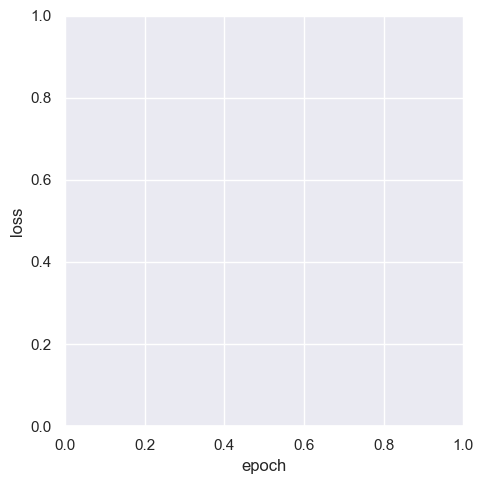
\includegraphics[width=.9\linewidth]{./.ob-jupyter/5e1419e04ffa8611806495b89d9dcbfafe0c4049.png}
\end{center}

\subsection{Sampling}
\label{sec:org98188c5}
We sample images from the trained DDPM model.
\begin{minted}[,frame=single, linenos, breaklines, tabsize=2]{python}
import matplotlib.pyplot as plt
import optax
from jax import random
import jax.numpy as jnp
from tqdm import tqdm

import utils
from unet import Unet

def sample(state, n, betas, key):
  # random white noise X_T
  key, subkey = random.split(key)
  x_k = random.normal(subkey, shape=(n, 28, 28, 1))

  #dts = np.array([ts[i] - ts[i-1] for i in range(1, steps+1)])
  #betas = 1- np.exp(-dts)
  alphas = 1 - betas
  alpha_bars = jnp.cumprod(alphas)
  #alpha_bars = jnp.array([alphas[:i+1].prod() for i in range(len(alphas))]) # workaround for metal problem with jnp.cumprod

  # sample in reverse from T=10 to 0.0 in evenly distributed steps
  #for i in tqdm(range(steps)[::-1]):
  for k in tqdm(range(len(betas))[::-1]):
    alpha = alphas[k]
    beta = betas[k]
    alpha_bar_k = alpha_bars[k]

    key, subkey = random.split(key)
    z = jnp.where(k > 1, random.normal(subkey, shape=x_k.shape), jnp.zeros_like(x_k))
    sigma_k = jnp.sqrt(beta) # option 1; see DDPM 3.2
    #sigma_k = jnp.sqrt((1-alpha_bars[k-1])/(1 - alpha_bar_k) * beta) # option 2; see DDPM 3.2

    x_k = 1/jnp.sqrt(alpha) * (x_k - beta/jnp.sqrt(1 - alpha_bar_k) * state.apply_fn(state.params, x_k, k * jnp.ones((x_k.shape[0], )))) + sigma_k * z

    x_k = jnp.clip(x_k, -1., 1.) # should we clip ...
    #x_t = normalize_to_neg_one_to_one(x_t) # or scale?

  return x_k

key = random.PRNGKey(SEED)

# use the best params
file_path, epoch, step, loss = utils.find_latest_pytree(f'{PROJECT_DIR}/ddpm_params_*.npy')
ddpm_state = utils.create_training_state(params_file=f'{PROJECT_DIR}/ddpm_params_{epoch}_{step}_{loss}.npy')
print(f'using parameters from epoch {epoch} with loss {loss}')

betas = jnp.linspace(MIN_BETA, MAX_BETA, K)

# generate x_0 from noise
key, subkey = random.split(key)
x_0_tilde = sample(ddpm_state, 4, betas, subkey)

# plot the data
utils.show_img_grid(utils.unnormalize_image(x_0_tilde))
\end{minted}

\begin{verbatim}
2024-03-07 08:56:45.170093: W external/xla/xla/service/gpu/nvptx_compiler.cc:742] The NVIDIA driver's CUDA version is 12.0 which is older than the ptxas CUDA version (12.4.99). Because the driver is older than the ptxas version, XLA is disabling parallel compilation, which may slow down compilation. You should update your NVIDIA driver or use the NVIDIA-provided CUDA forward compatibility packages.
using parameters from epoch 8 with loss 0.02443
100% 1000/1000 [14:06<00:00,  1.18it/s]
\end{verbatim}

\begin{center}
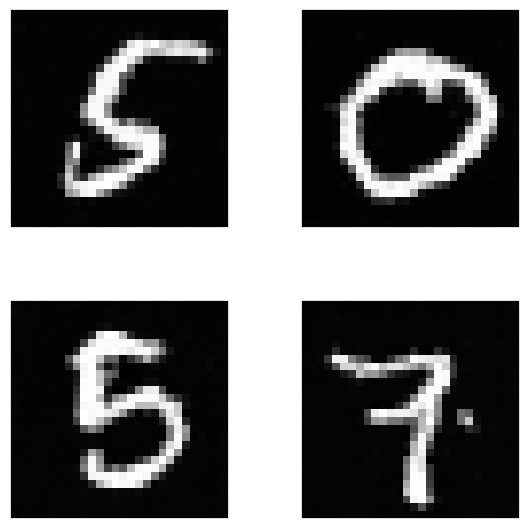
\includegraphics[width=.9\linewidth]{./.ob-jupyter/366e5ecd5190dcfa0dfd0afc39a52d418f35ab5e.png}
\end{center}

\section{CEM}
\label{sec:orgfb93212}
\begin{minted}[,frame=single, linenos, breaklines, tabsize=2]{python}
import os

SEED=42
T=10.
K=1000
BATCH_SIZE = 1000
PROJECT_DIR=os.path.abspath('.')
\end{minted}
\subsection{Training}
\label{sec:org884c05e}
Training is performed via a python script \url{train\_cem.py}. We examine the average epoch loss with the following code:
\begin{minted}[,frame=single, linenos, breaklines, tabsize=2]{python}
import pandas as pd
import matplotlib.pyplot as plt
import seaborn as sns

import utils

cem_loss_log = utils.load_loss_log(f'{PROJECT_DIR}/cem_loss_log.npy')

# plot losses
df = pd.DataFrame([(int(x), float(y)) for x, _, y in cem_loss_log], columns=['epoch', 'loss'])
sns.relplot(df, x='epoch', y='loss', kind='line')

_ = plt.tight_layout()
_ = plt.show()
\end{minted}

\begin{center}
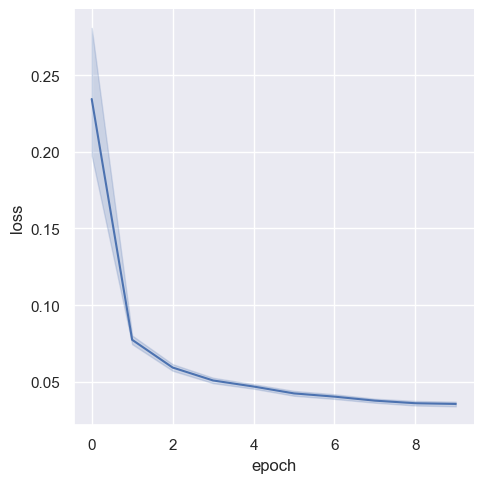
\includegraphics[width=.9\linewidth]{./.ob-jupyter/6a99d9467be35764e879e334f59da6c04468e95f.png}
\end{center}

\subsection{Sampling}
\label{sec:orgc76281b}
We sample images from the trained CEM model.
\begin{minted}[,frame=single, linenos, breaklines, tabsize=2]{python}
import matplotlib.pyplot as plt
import optax
from jax import random
import jax.numpy as jnp
from tqdm import tqdm

import utils
from unet import Unet

def sample(state, n, ts, key):
  # random white noise X_T
  key, subkey = random.split(key)
  x_t = random.normal(subkey, shape=(n, 28, 28, 1))

  step=0

  for k in tqdm(range(len(ts))[::-1]):
    key, subkey = random.split(key)
    z = random.normal(subkey, shape=x_t.shape)

    t = ts[k]
    dt = jnp.where(k > 0, t - ts[k-1], 0.)

    f_theta = state.apply_fn(state.params, x_t, t * jnp.ones((n,)))

    # equation (40)
    s_theta = jnp.where(k > 0, x_t/(1-jnp.exp(-t))  - jnp.exp(-t/2)/(1-jnp.exp(-t)) * f_theta,  0.)

    # equation (24)
    x_t_bar = x_t - dt * s_theta
    x_t = jnp.exp(dt/2) * x_t_bar + jnp.sqrt(1-jnp.exp(-dt)) * z

    x_t = jnp.clip(x_t, -1., 1.) # should we clip ...
    #x_t = normalize_to_neg_one_to_one(x_t) # or scale?

    step=step+1

  return x_t

key = random.PRNGKey(SEED)

# use the best params
file_path, epoch, step, loss = utils.find_latest_pytree(f'{PROJECT_DIR}/cem_params_*.npy')
cem_state = utils.create_training_state(params_file=f'{PROJECT_DIR}/cem_params_{epoch}_{step}_{loss}.npy')
print(f'using parameters from epoch {epoch} with loss {loss}')

ts = utils.exponential_time_schedule(T, K)

# generate x_0 from noise
key, subkey = random.split(key)
x_0_tilde = sample(cem_state, 16, ts, subkey)

# plot the data
utils.show_img_grid(utils.unnormalize_image(x_0_tilde))
\end{minted}

\begin{verbatim}
using parameters from epoch 9 with loss 0.03557
100% 1002/1002 [09:41<00:00,  1.72it/s]

\end{verbatim}

\begin{center}
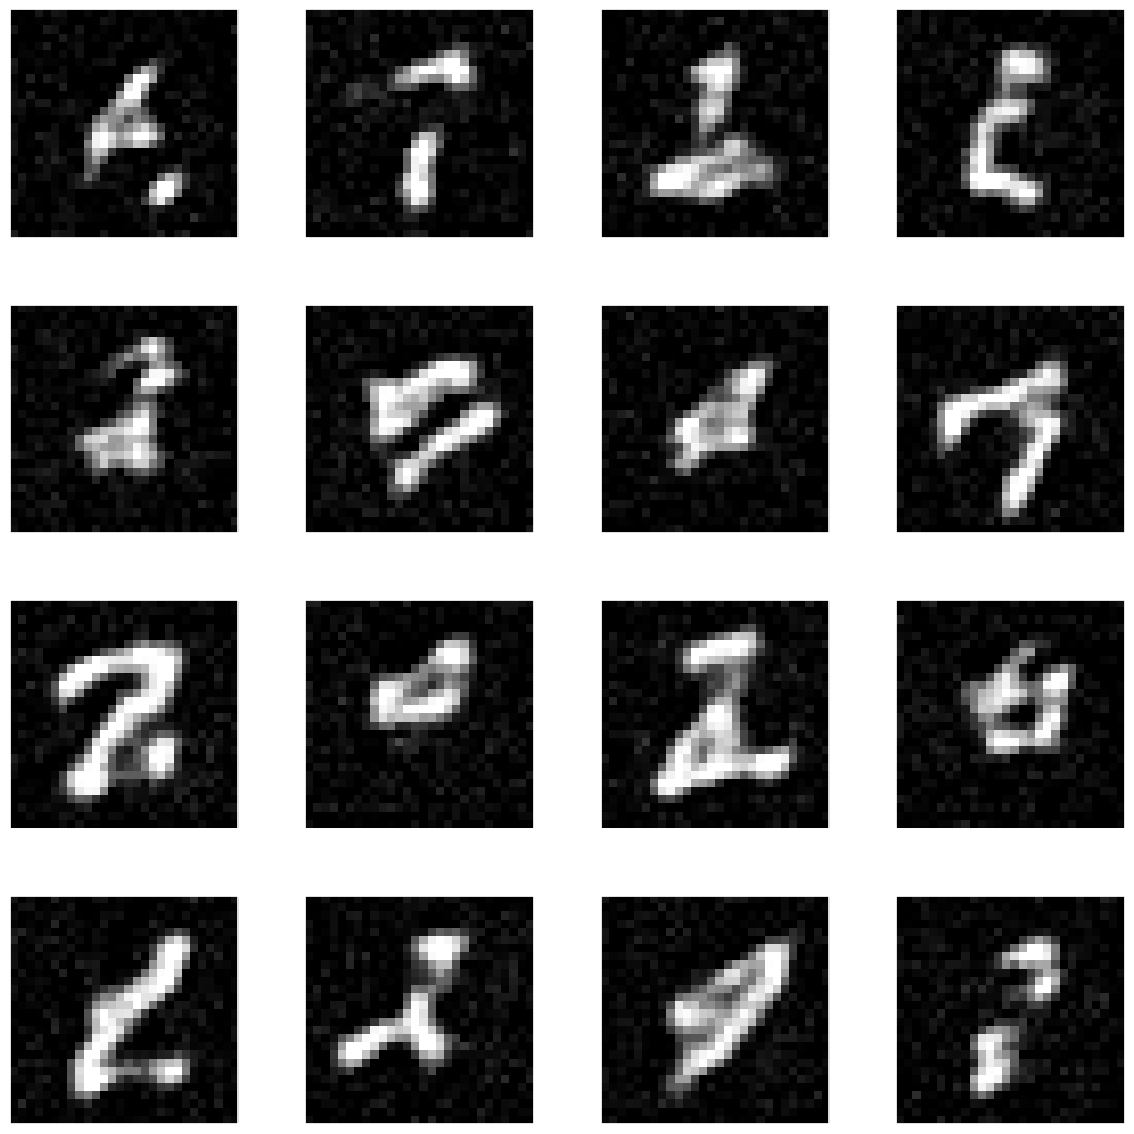
\includegraphics[width=.9\linewidth]{./.ob-jupyter/0f3f0e54e530983abb7d269c4c35266ac2b88c7c.png}
\end{center}

\section{Reads}
\label{sec:org1c1e5e4}
\begin{itemize}
\item Quick summary on CR reconstruciton and Helical CT \url{http://xrayphysics.com/ctsim.html}
\item Example to perform simple image reconstruction using scikit-image \url{https://scikit-image.org/docs/stable/auto\_examples/transform/plot\_radon\_transform.html}
\item Python code to reconstruct image from helical scans? \url{https://github.com/dzwiedzn7/filtered-back-projection/blob/master/tompy.py}
\item Python code to simulate thick slice images from Helical scans \url{https://github.com/Feanor007/Thin2Thick}
\item Python library for Tomography \url{https://pypi.org/project/algotom/}
\item C code for Model-Based Iterative Reconstruciton code for Multi-Slice Helical Geometry \url{https://github.com/cabouman/OpenMBIR-Index/blob/master/README.md}
\item General summary for 3D image reconstruction \url{https://humanhealth.iaea.org/HHW/MedicalPhysics/NuclearMedicine/ImageAnalysis/3Dimagereconstruction/index.html}
\item Pyro-NN: Generalized Python code for image reconstruction using deep learning implemented in Tensorflow code \url{https://www.ncbi.nlm.nih.gov/pmc/articles/PMC6899669/}
\item TomoPy: python library for tomographic data analysis \url{https://www.ncbi.nlm.nih.gov/pmc/articles/PMC4181643/}
\item Powerpoint presentation on CT image reconstruction \url{http://www.sci.utah.edu/\~shireen/pdfs/tutorials/Elhabian\_CT09.pdf}
\item Astra toolbox: python matlab library for 2D/3D tomography \url{https://github.com/astra-toolbox/astra-toolbox}
\item Operator Discretization Library (ODL): used by authors of the paper and has example Python code to reconstruct image from Helical scans \url{https://github.com/odlgroup/odl/tree/master/examples/tomo}
\item matlab code for simple low-dose CT samples simulation \url{https://github.com/smuzd/LD-CT-simulation/tree/master}
\item matlab code for 2nd winner from 2016 Mayo Grand Challenge \url{https://github.com/jongcye/deeplearningLDCT/tree/master}
\item Jupyter code to add white noise to CT scans. May have code to reconstruct images from Helical scans? \url{https://github.com/ayaanzhaque/Noise2Quality}
\item Alternative CT training data? \url{https://www.kaggle.com/c/data-science-bowl-2017/overview}
\item Alternative CT training data from piglets? \url{https://link.springer.com/article/10.1007/s10278-018-0056-0}
\end{itemize}
\section{References}
\label{sec:org48d6488}
\noindent
Adler, Jonas and Öktem, Ozan (2018). \emph{Deep {{Bayesian Inversion}}}.

\noindent
McCollough, Cynthia H. and Bartley, Adam C. and Carter, Rickey E. and Chen, Baiyu and Drees, Tammy A. and Edwards, Phillip and Holmes, David R. and Huang, Alice E. and Khan, Farhana and Leng, Shuai and McMillan, Kyle L. and Michalak, Gregory J. and Nunez, Kristina M. and Yu, Lifeng and Fletcher, Joel G. (2017). \emph{Low-Dose {{CT}} for the Detection and Classification of Metastatic Liver Lesions: {{Results}} of the 2016 {{Low Dose CT Grand Challenge}}}.

\noindent
Moen, Taylor R. and Chen, Baiyu and Holmes III, David R. and Duan, Xinhui and Yu, Zhicong and Yu, Lifeng and Leng, Shuai and Fletcher, Joel G. and McCollough, Cynthia H. (2021). \emph{Low-Dose {{CT}} Image and Projection Dataset}.

\noindent
Yi, Xin and Babyn, Paul (2018). \emph{Sharpness-Aware {{Low}} Dose {{CT}} Denoising Using Conditional Generative Adversarial Network}.

\noindent
Zeng, Dong and Huang, Jing and Bian, Zhaoying and Niu, Shanzhou and Zhang, Hua and Feng, Qianjin and Liang, Zhengrong and Ma, Jianhua (2015). \emph{A {{Simple Low-dose X-ray CT Simulation}} from {{High-dose Scan}}}.
\end{document}
